CrowdNote is an environment that can be modified to become different kinds of crowdsourcing applications based on video annotations. To create a system based on this environment is required to define the required tasks, the aggregation methods that should be applied to each task, and create the simple annotation tools for each task.

To demonstrate its working was built an instance of CrowdNote which consists of a system for video enrichment by adding extra content provided by the crowd. In this system, contributors are responsible for identifying the points of interest in the video, suggesting that the content is associated with each one, deciding the best suggestion for each point of interest, and finally deciding the best position in the video to present each content.

The extra content suggested by the crowd are images, text boxes, Wikipedia content, and Youtube videos, and the result delivered by this system is an enriched video, that consists of the original video presented synchronized with the extra content provided and selected by the crowd. 

The approach taken to achieve the complex annotation needed to enrich the videos is to cascade microtasks that collect simple annotations, instead of collecting complex annotations for each contribution. In this way, people without specialization or training can contribute to the process.


\begin{itemize}
\item \textbf{Task 1 - Identify the points of interest} in the video that should be associated with the extra content. The first microtask is to send video segments to the worker and ask him to identify in this segment something that he believes deserves to be highlighted or supplemented. The aggregation rules for this microtask are to temporarily group the annotations with a tolerance of 0.5 sec, to count and to merge similar annotations in each group, and to determine for each time group which is the predominant point of interest in the annotations.

\item \textbf{Task 2: Provide extra content suggestions} for each point of interest. In the second task, the worker receives a point of interest and should to suggest extra content related to it. This content can be a text, an image, a YouTube video or a Wikipedia page. The aggregation of the second task consists in grouping the contributions by a point of interest and joining similar contributions to avoid duplicity.

\item \textbf{Task 3: Ranking the suggested content} provided by each point of interest. In the third microtask, the worker receives a point of interest and the content suggestions for it. The contributor should choose the most appropriate content for the point presented. The aggregation rule for this task is to select the most popular content for each point of interest.
	
\item \textbf{Task 4: Determine the positions} to display the extra content associated with each point of interest. In this task, the worker receives an item that represents a point of interest and chooses the position in the video most suitable to display it. The aggregate for this task calculates the average coordinate for each item to be displayed in the video.

\end{itemize}

\pagebreak


\subsection{Cascading Microtasks}
The adopted approach consists in divide the complex annotation into simple annotations that can be collected by 
a set of simple annotation tools. Each of these simple annotations is collected by a microtask.

How is illustrated in Figure~\ref{cascading}, the input for each task is generated by the Aggregator after the previous task, except for the task 1. For this task is provided a bootstrap Input that is a list of video segments provided by the owner, that is who initiate the process. Each entry of the bootstrap input can represent a semantic block of the video. 

\begin{figure}[h!]
 \centerline{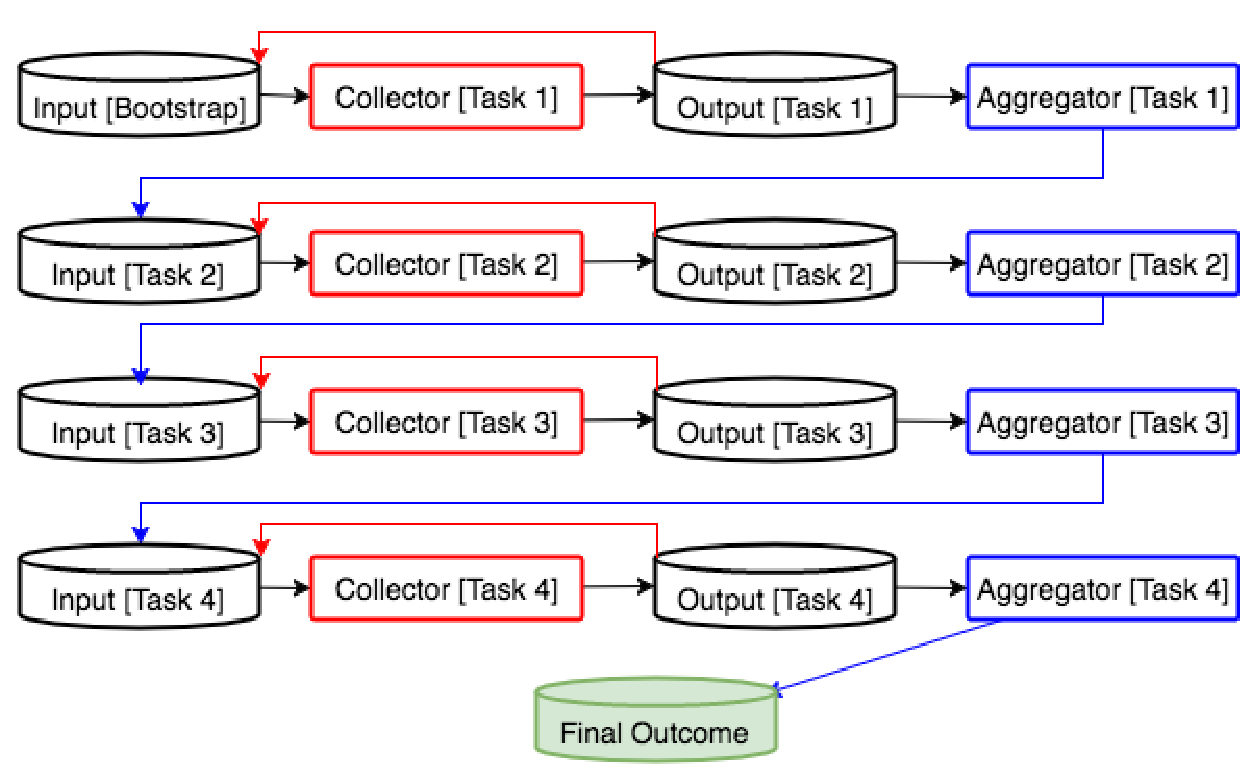
\includegraphics[scale=0.35] {figure/Cascading}}
	\caption{Cascading Microtasks}
	\label{cascading}
\end{figure}

Other applications that use CrowdNote may use different strategies to segment videos such as fixed time-length, SRT files, or even add a microtask to segment videos.
		


\subsection{Task 1}
\textbf{Identify Points of Interest:} The first annotation microtask is supported by the tool represented in Figure~\ref{task_1}, collecting identification for points of interest. In this task, the contributor receives a segment of video that should be watched, and if was found any point of interest, it should be marked and briefly described. These points of interest can be gestures, words, expressions, facts, concept, characters, events or anything that can be related to extra content.

\begin{figure}[h!]
	\centerline{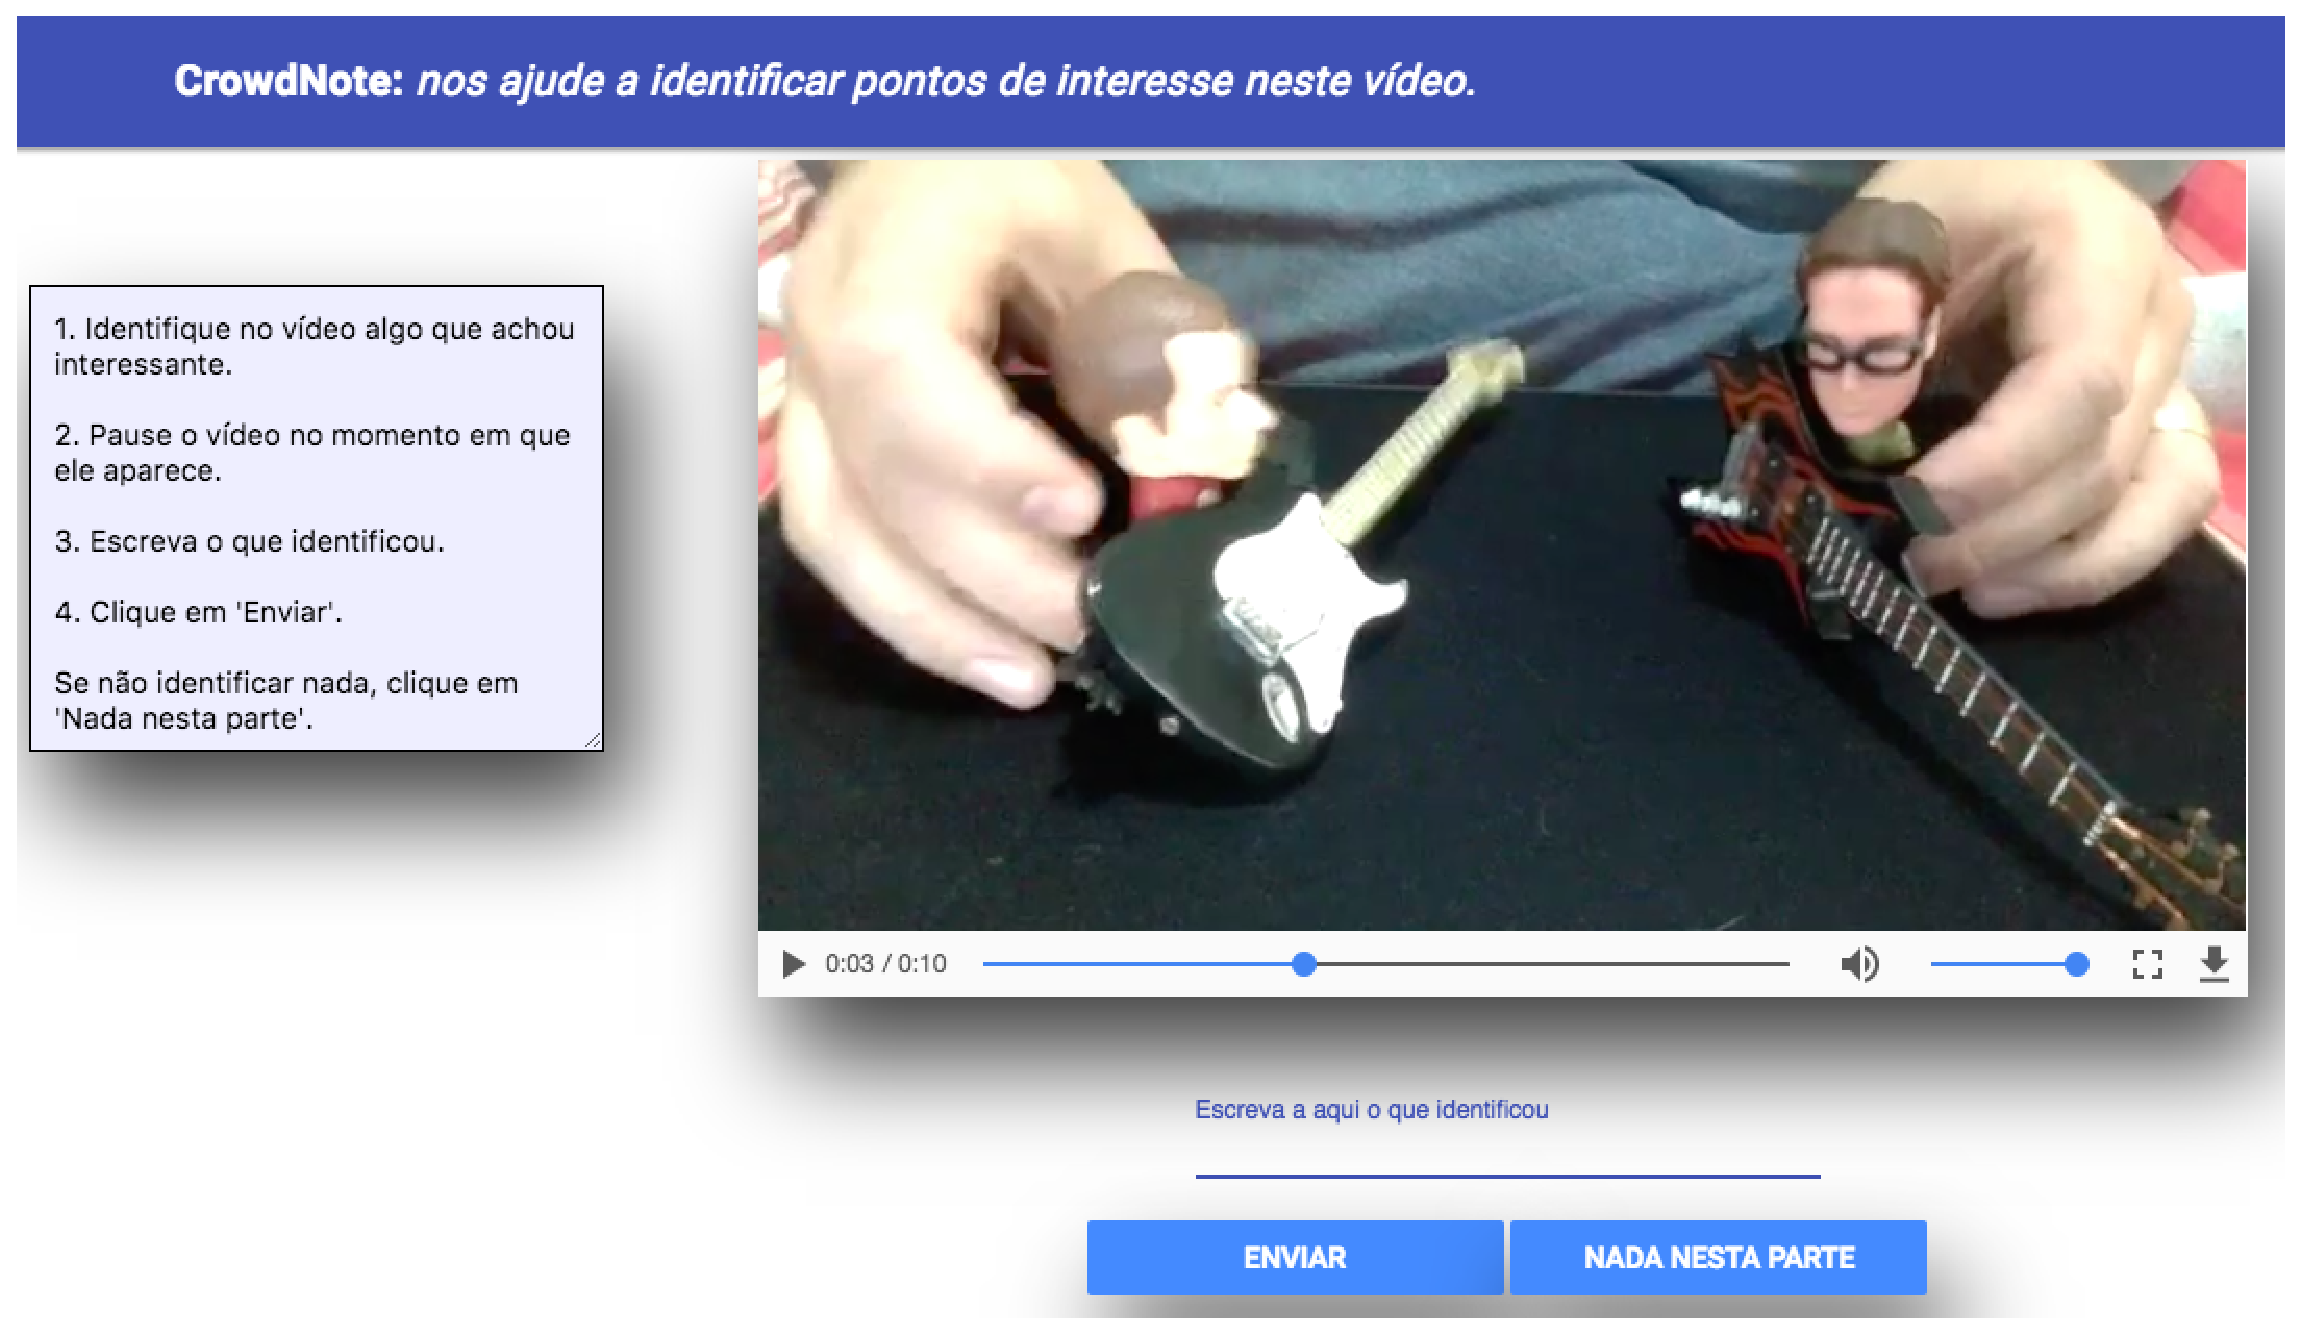
\includegraphics[scale=0.22] {figure/task_1}}
	\caption{Annotation Tool for Task 1}
	\label{task_1}
\end{figure}

\subsection{Task 2}

\textbf{Provide extra content suggestions:} The second task took as input the aggregated result from the task 1 that is a list of points of interest identified by the workers. This microtask is supported by the annotation tool represented in Figure~\ref{task_2}. This tool presents the worker a point of interest and the video segment positioned at the moment it occurs. This way, you can use video for reference and contextualization.

Through this tool, the worker can contribute by writing a text related to the point of interest, sending an image or sending a link to a YouTube video or a Wikipedia page.

\begin{figure}[h!]
	\centerline{\includegraphics[scale=0.18] {figure/task_2}}
	\caption{Annotation Tool for Task 2}
	\label{task_2}
\end{figure}

When you close the collection of contributions for this task, the Aggregator groups the content of the sender by a point of interest, and then joins the similar suggestions. In this way, a list of points of interest with a set of content suggestions for each is added to the next task, without repeated suggestions.


\subsection{Task 3}

\textbf{Ranking Suggestions:} The third task receives as input the list of points of interest, with the content suggestions for each of them. For each job, the annotation tool illustrated in Figure~\ref{task_3} shows the worker a point of interest and the video positioned at the time that point occurs. The annotation tool displays the content suggestions for that point of interest below the video, so you can browse through the content to choose the most appropriate one.

\begin{figure}[h!]
	\centerline{\includegraphics[scale=0.22] {figure/task_3}}
	\caption{Annotation Tool for Task 3}
	\label{task_3}
\end{figure}

The worker can enlarge each content to see it better, how can be seen in Figure~\ref{zoom_task_3}. In addition to playing the videos as a suggestion of content.		
		
\begin{figure}[h!]
	\centerline{\includegraphics[scale=0.18] {figure/zoom_t3}}
	\caption{Annotation Tool for Task 3 - Zoom}
	\label{zoom_task_3}
\end{figure}

The aggregation process for this task counts the votes for each content suggestion and chooses the most popular content for each point of interest.



\subsection{Task 4}

\textbf{Determine the positions:} The last task receives as input the list of points of interest and the content chosen to associate with it. For each job, the tool shown in Figure~\ref{task_4} shows the worker the video that is positioned at the time the point of interest occurs and the reference item for the content selected in the video.

The contribution to this task is to suggest the best position to present the extra content, using the annotation tool to determine this position. The tool allows the worker to change the position of the item in the video by clicking the desired point. Among the 4 microtasks, this is the fastest and easiest to perform.

\begin{figure}[h!]
	\centerline{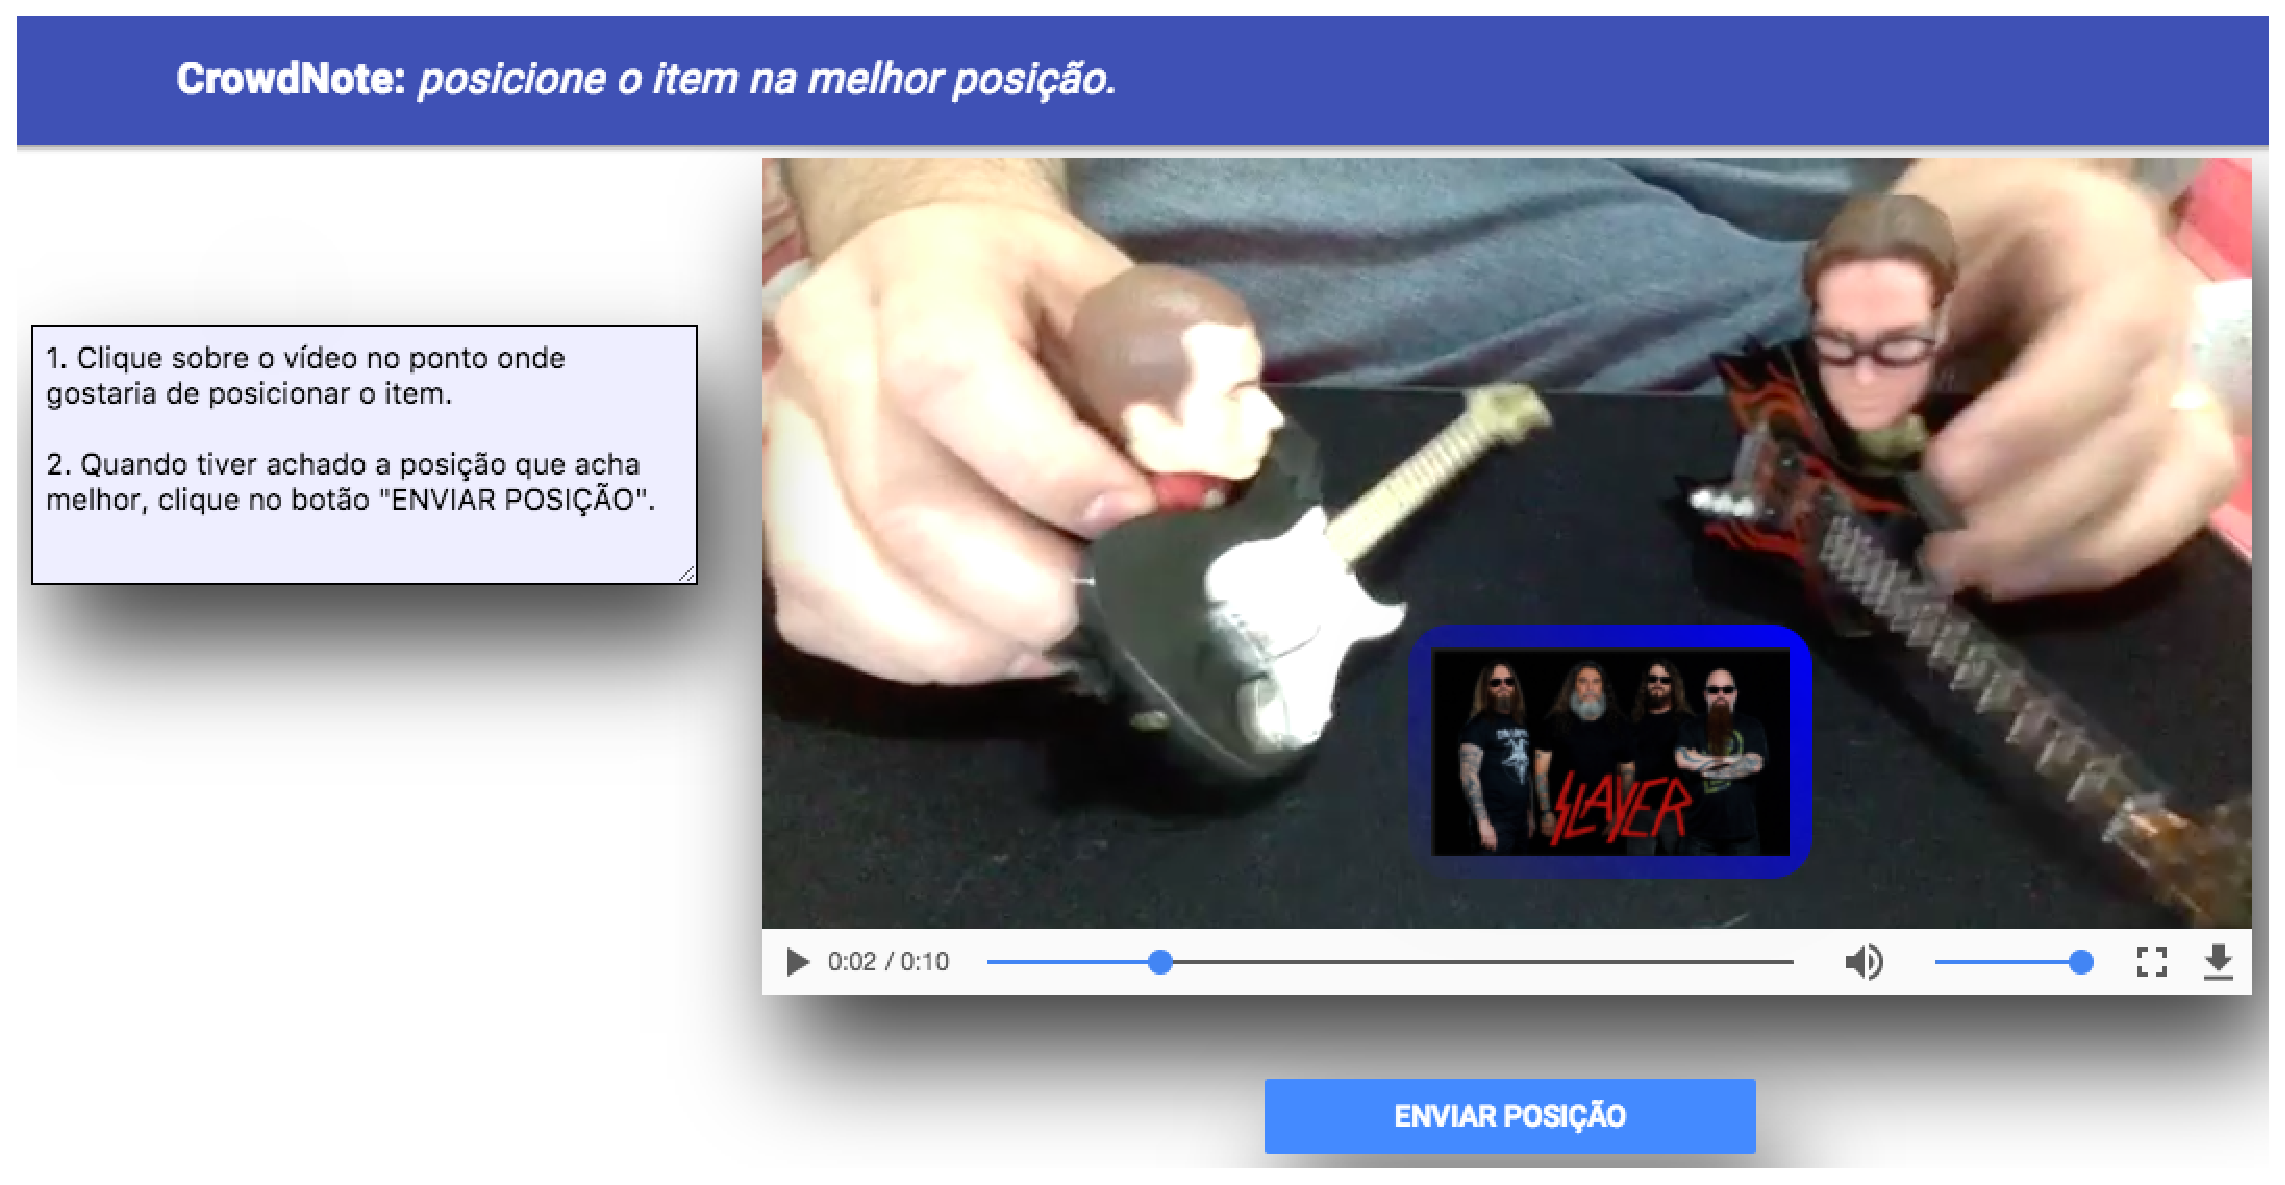
\includegraphics[scale=0.22] {figure/task_4}}
	\caption{Annotation Tool for Task 4}
	\label{task_4}
\end{figure}

Following the studies about the wisdom  of the crowd, the strategy to determine the correct position is to calculate the average coordinate of the contribution for each content \citep{GALTON1907}. In this way, the aggregation process calculates the average coordinate of the items, based on the contributions of the crowd. The result of this process is the position where each item related to a point of interest that will appear in the video.


\pagebreak

\subsection{Player}

The presentation system, shown in Figure~\ref{player}, receives the video, extra content, and necessary meta-data from the Player Provider. This system is capable of reproducing the original video synchronized with the extra content, that is displayed every time a point of interest happens in the video. Is important to remind that all extra content displayed with the video was provided, selected and positioned by the crowd.

\begin{figure}[h!]
	\centerline{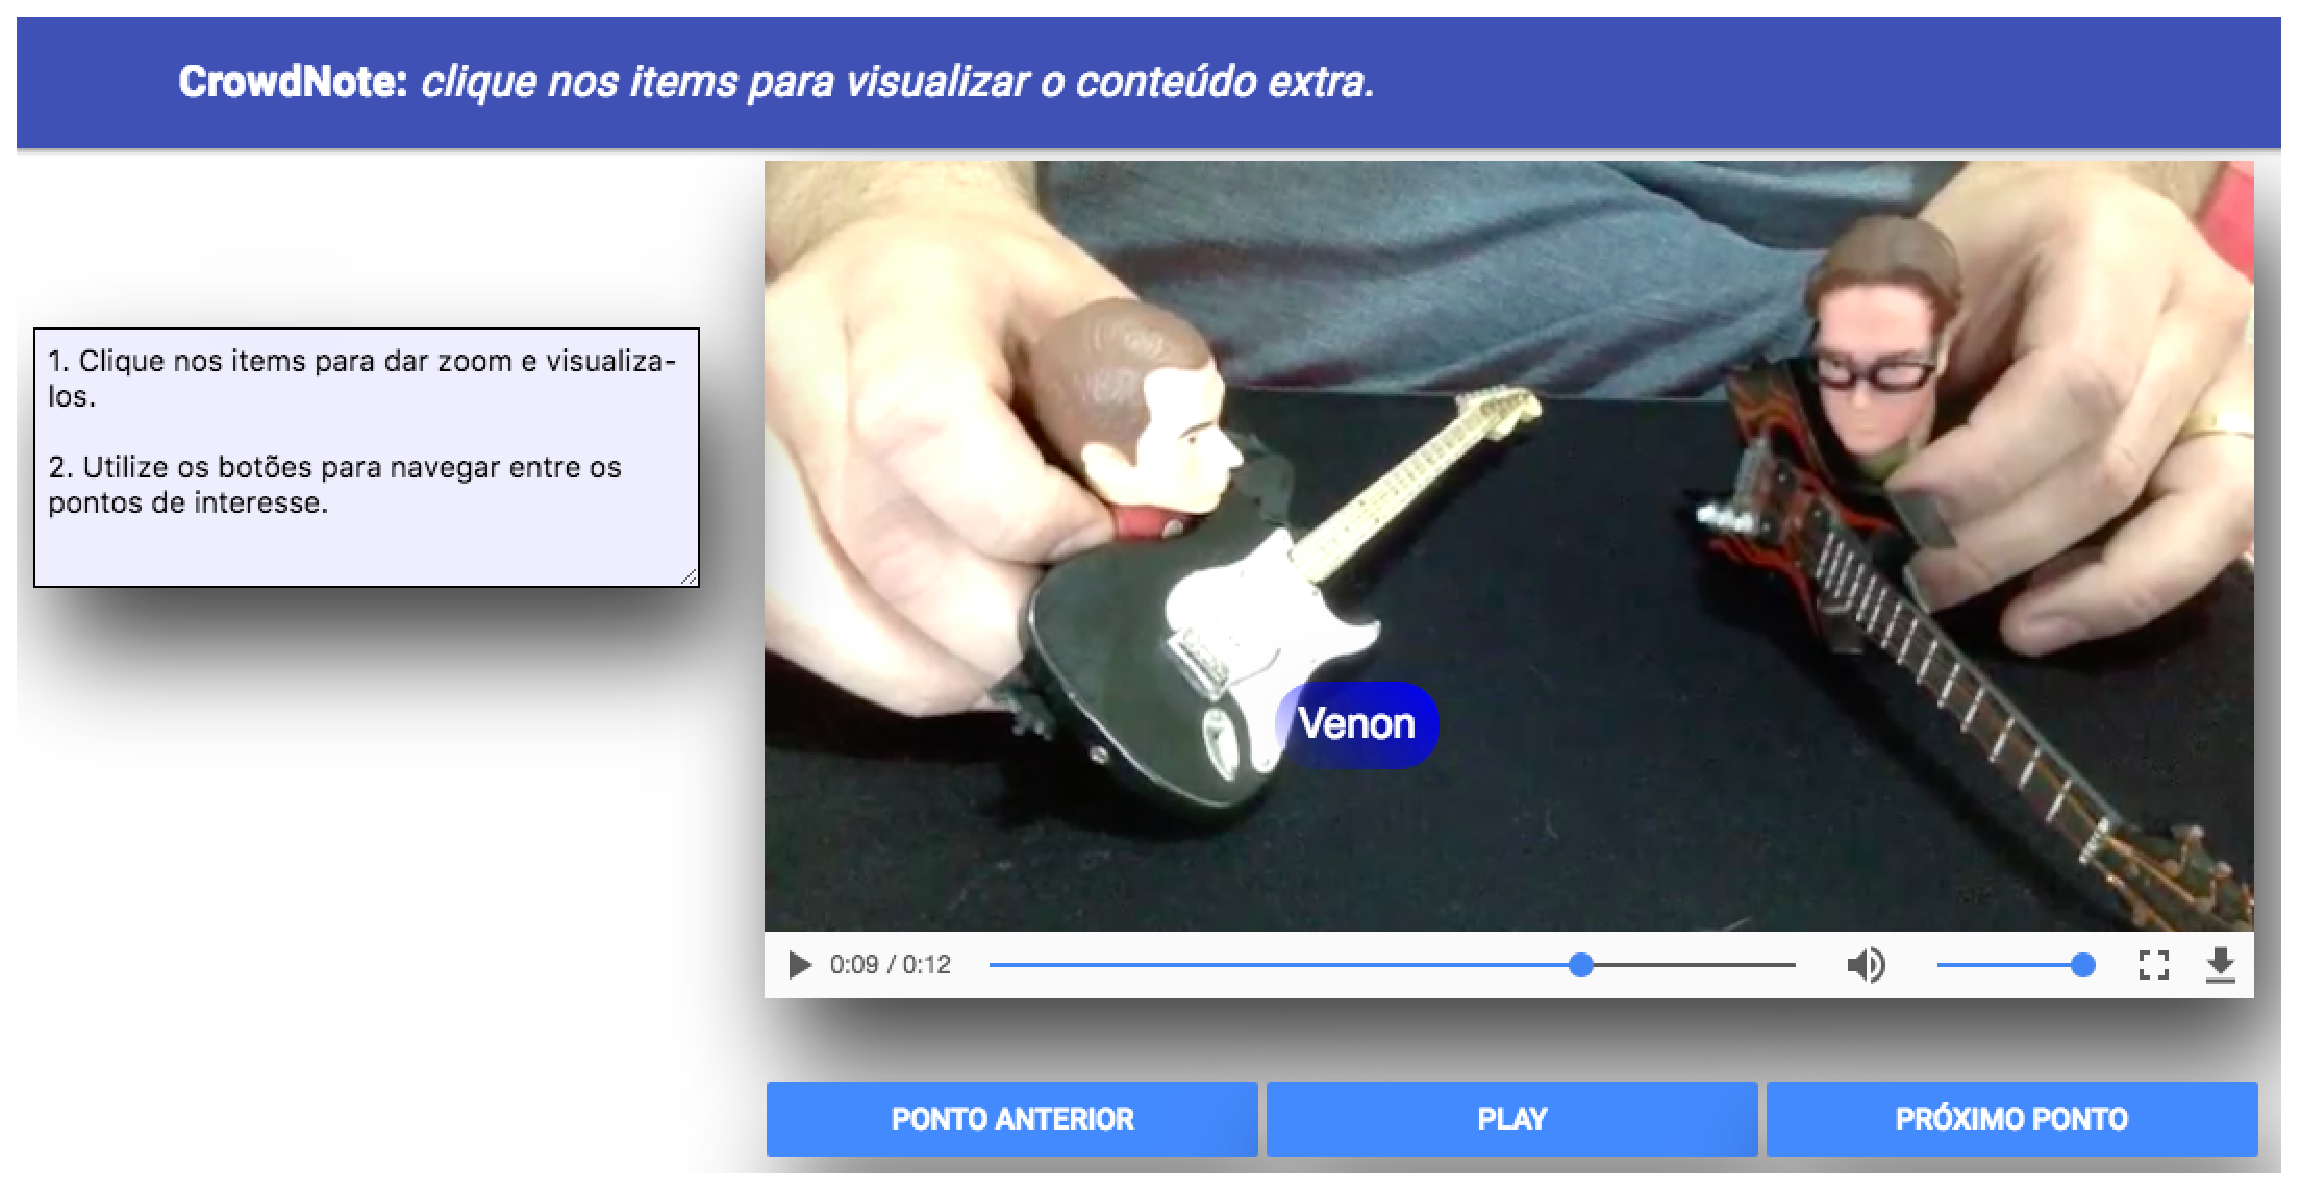
\includegraphics[scale=0.22] {figure/player}}
	\caption{Displaying an extra content item over the video}
	\label{player}
\end{figure}

When the user clicks on some extra content displayed in the video, the presentation is paused and a larger preview of the selected content is displayed in the zoom box as shown in Figure~\ref{zoom}. This system features navigation by extra-content instead the traditional timeline navigation, making available a button-bar with buttons to navigate among the extra contents.
 
\begin{figure}[h!]
	\centerline{\includegraphics[scale=0.18] {figure/zoom}}
	\caption{Displaying an extra content into a zoom modal}
	\label{zoom}
\end{figure}
